\section{gyro\_\-spi.h File Reference}
\label{gyro__spi_8h}\index{gyro_spi.h@{gyro\_\-spi.h}}
{\tt \#include $<$inttypes.h$>$}\par


Include dependency graph for gyro\_\-spi.h:\begin{figure}[H]
\begin{center}
\leavevmode
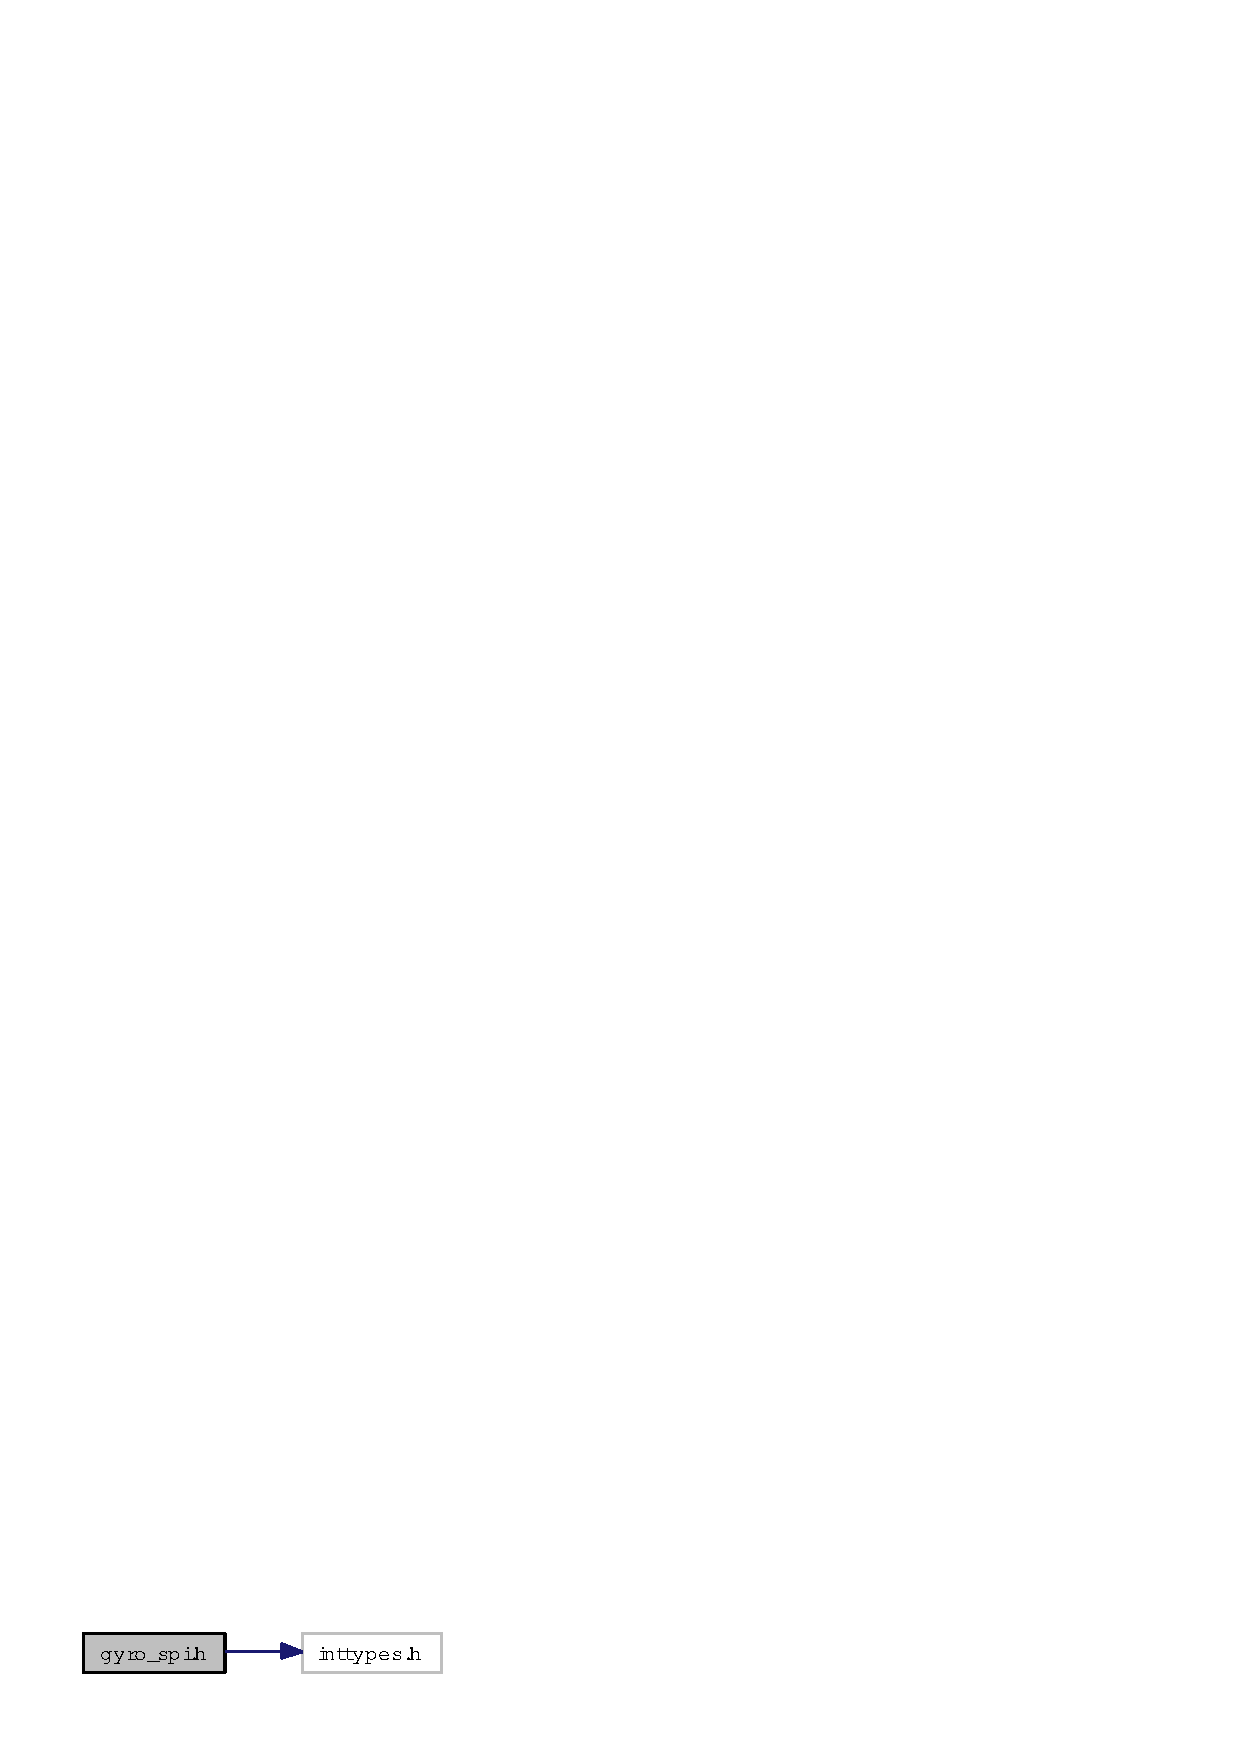
\includegraphics[width=108pt]{gyro__spi_8h__incl}
\end{center}
\end{figure}


This graph shows which files directly or indirectly include this file:\begin{figure}[H]
\begin{center}
\leavevmode
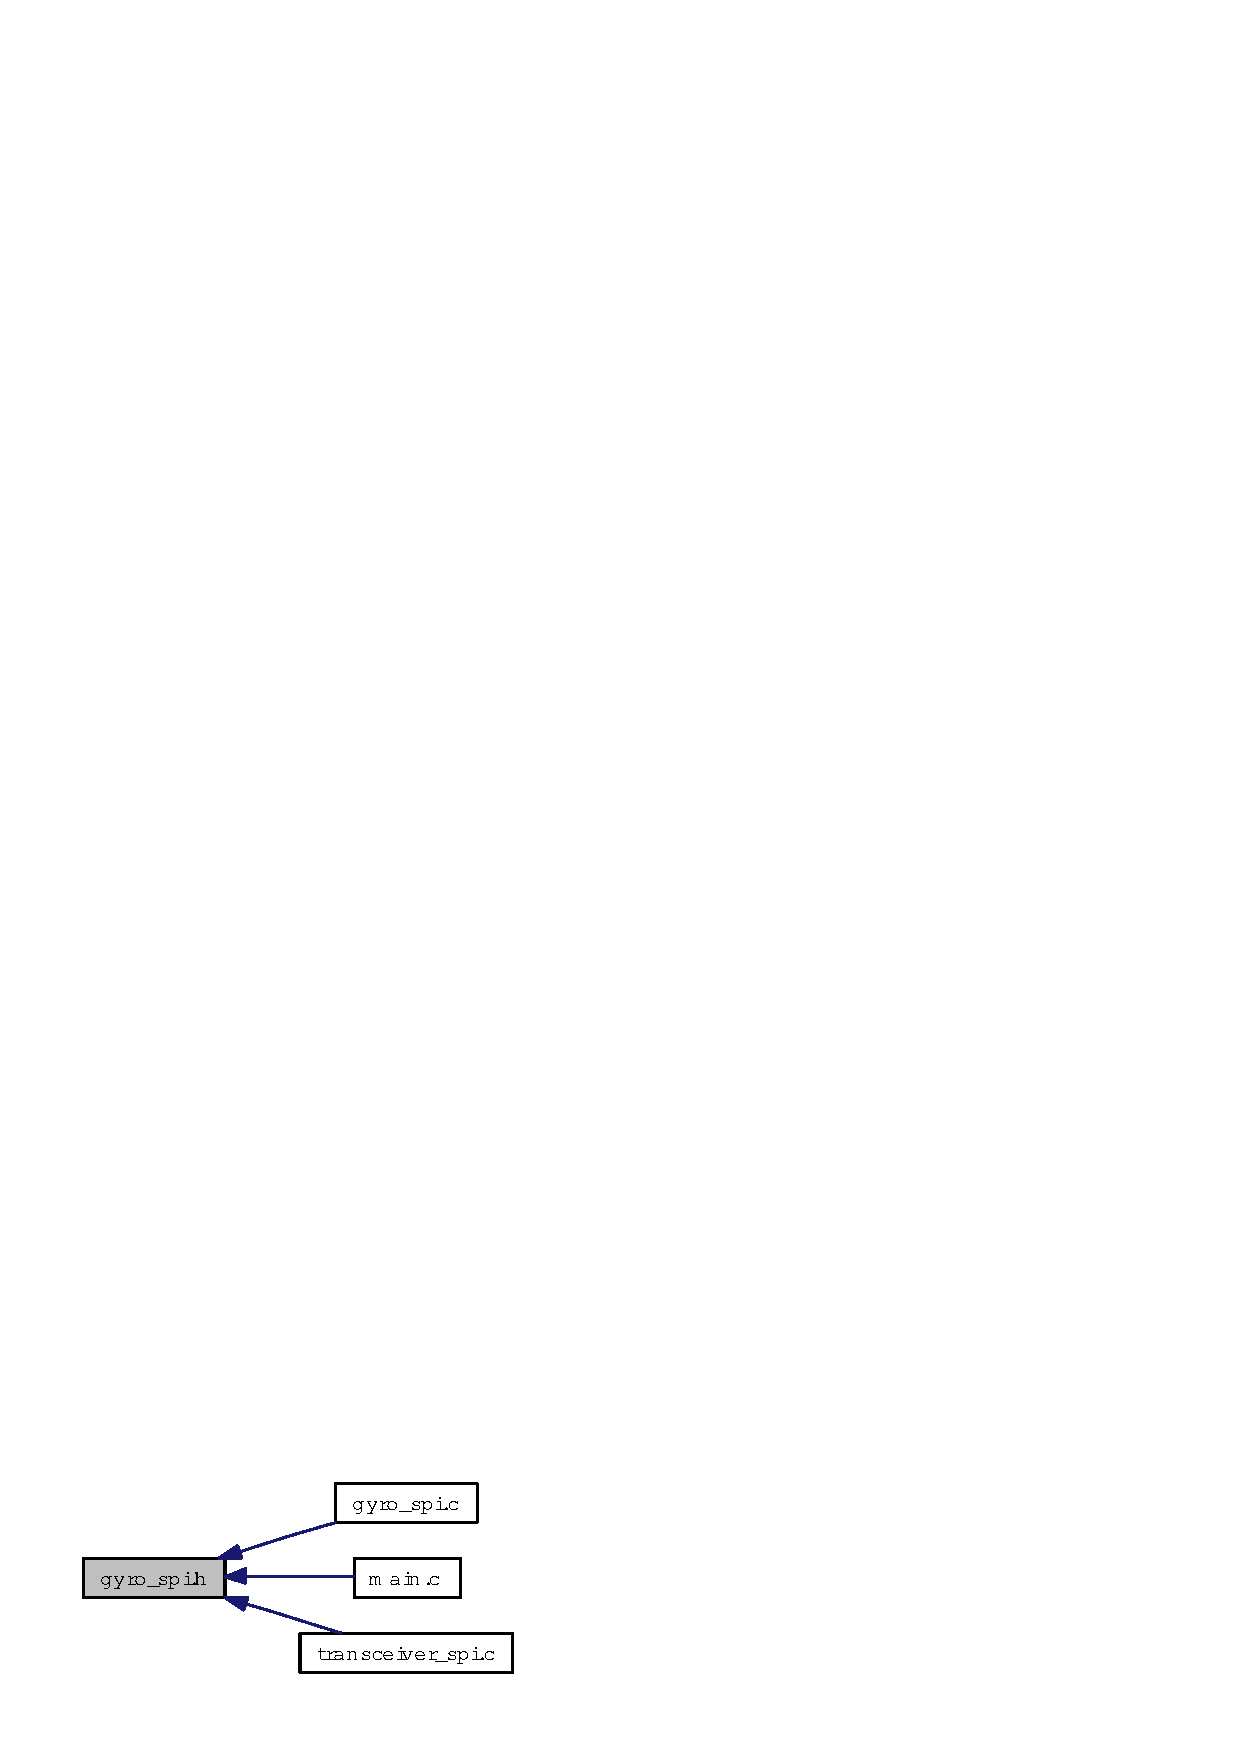
\includegraphics[width=125pt]{gyro__spi_8h__dep__incl}
\end{center}
\end{figure}
\subsection*{Defines}
\begin{CompactItemize}
\item 
\#define {\bf CS\_\-GYRO1}~0
\item 
\#define {\bf CS\_\-GYRO2}~2
\item 
\#define {\bf ACC\_\-HB}~0x83
\item 
\#define {\bf ACC\_\-LB}~0x00
\item 
\#define {\bf TEMP\_\-HB}~0x87
\item 
\#define {\bf TEMP\_\-LB}~0x00
\end{CompactItemize}
\subsection*{Typedefs}
\begin{CompactItemize}
\item 
typedef enum {\bf gyro\_\-fsm\_\-state\_\-enum} {\bf gyro\_\-fsm\_\-state}
\end{CompactItemize}
\subsection*{Enumerations}
\begin{CompactItemize}
\item 
enum {\bf gyro\_\-fsm\_\-state\_\-enum} \{ \par
{\bf first\_\-run}, 
{\bf g1\_\-hacc}, 
{\bf g1\_\-lacc}, 
{\bf g2\_\-hacc}, 
\par
{\bf g2\_\-lacc}, 
{\bf g1\_\-htmp}, 
{\bf g1\_\-ltmp}, 
{\bf g2\_\-htmp}, 
\par
{\bf g2\_\-ltmp}
 \}
\end{CompactItemize}
\subsection*{Functions}
\begin{CompactItemize}
\item 
void {\bf init\_\-spi\_\-gyro} (uint8\_\-t interrupt\_\-mode)
\item 
void {\bf spi\_\-cs} (uint8\_\-t chip)
\item 
uint8\_\-t {\bf spi\_\-write\_\-8} (uint8\_\-t data)
\begin{CompactList}\small\item\em Transfer 1 Byte given in data via the SPI return the 1 Byte sampled during transfer. \item\end{CompactList}\item 
uint8\_\-t {\bf spi\_\-write\_\-8\_\-nocs} (uint8\_\-t data)
\item 
uint16\_\-t {\bf spi\_\-write\_\-16} (uint16\_\-t data)
\begin{CompactList}\small\item\em Tranfer 2 Bytes given in data via the SPI, return the 2 Bytes sampled during transfer. \item\end{CompactList}\item 
uint16\_\-t {\bf spi\_\-write\_\-16\_\-nocs} (uint16\_\-t data)
\end{CompactItemize}
\subsection*{Variables}
\begin{CompactItemize}
\item 
{\bf gyro\_\-fsm\_\-state} {\bf gyro\_\-state}
\end{CompactItemize}
